\chapter{Unconstrained optimization}
Optimization is the search for a minimum or maximum of some objective function. In fact, we can focus on minimization only, because maximization can be transferred to minimization by multiplying the objective function with $-1$. 
We are familiar with such problems from basic math courses in which we learned that the minimum of a continuous differentiable function $f(x)$ fulfills the necessary condition $f'(x)=0$ and the sufficient condition $f''(x) > 0$. 

Here, we extend this concept to a multi-dimensional optimization variable $\mathbf{x} \in \mathcal{R}^d$ and formulate the optimization problem as 
\begin{equation}
    \min_{\mathbf{x}} \quad f(\mathbf{x})
   \label{eq:unconstrained_optimzation}
\end{equation}
with $f: \mathcal{R}^d \rightarrow \mathcal{R}$.

We may use an analogy at this point: \emph{Consider a person hiking in the mountains and the height of the mountains is described by a function $f$ that depends on the location $\mathbf{x}$. The person can go anywhere in the mountain range $\mathcal{R}^d$ without restrictions, but wants to get back to the village, which is located at the bottom of the deepest valley at position $\mathbf{x}^*$. To get to the location of that village, the person needs to solve Equation \eqref{eq:unconstrained_optimzation}.}

\begin{objectives}{}{objectives_unconstrained_optimization}
After studying this chapter and finishing the exercise, you should be able to 
\begin{itemize}[label=$\dots$]
    \item distinguish the local and global optimum
    \item define convexity of sets and functions
    \item explain gradient decent methods such as simple steepest decent, steepest decent with incomplete line search, conjugated gradients, and quasi Newton 
    \item implement these gradient decent methods in computer code
\end{itemize}
\end{objectives}

\section{Local and global optimum}
As mentioned earlier, we may interpret the problem \eqref{eq:unconstrained_optimzation} as searching for the lowest point $\mathbf{x}^* \in \mathcal{R}^d$ in a mountainous landscape, as illustrated in Figure \ref{fig:global_local_optimization}. 

This lowest point is termed \emph{global minimum}, if 
\begin{equation}
    f(\mathbf{x}^*) \le f(\mathbf{x})  \quad \forall \mathbf{x} \in \mathcal{R}^d.
\end{equation}
However, finding this global minimum is generally a challenging task, because it is computationally demanding to test all points against all other points. 

\begin{figure}
    \centering
    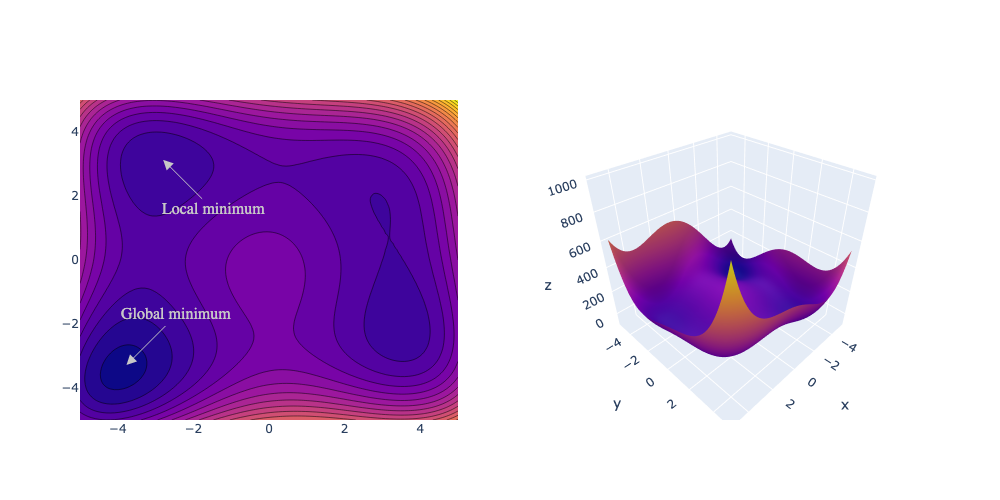
\includegraphics[width=\textwidth, alt={Optimization Landscape}]{figures/opti_landscape.png}
    \caption{Global and local optimum in an optimization problem.}
    \label{fig:global_local_optimization}
\end{figure}

Hence, we focus on the easier problem of trying to find \emph{local minima}, i.e. points which are lower or equal in a local neighborhood. A local minimum is located at a stationary point 
\begin{equation}
    \nabla f(\mathbf{x}^*) = \mathbf{0},
    \label{eq:stationary_point}
\end{equation}
even though not all stationary points are local minima (they could be a maximum or saddle points).
Of course, the global minimum is also a local minimum, but under which conditions is the local minimum also a global minimum? The answer to this question is "in \emph{convex problems}" and is explored in the next section.

\section{Convexity}
A set $\mathcal{S} \subset \mathcal{R}^d$ is termed \emph{convex}, if 
\begin{equation}
    \lambda \hat{\mathbf{x}} + (1-\lambda) \check{\mathbf{x}} \in \mathcal{S} \quad \forall \hat{\mathbf{x}}, \check{\mathbf{x}} \in \mathcal{S} \quad  \forall \lambda \in [0,1].
\end{equation}
This means, we are able to draw a straight line from any point in the set to another point in the set, in which any point at the line is still in the set (see Figure \ref{fig:convex_sets}).

\begin{figure}[!htpb]
    \centering
    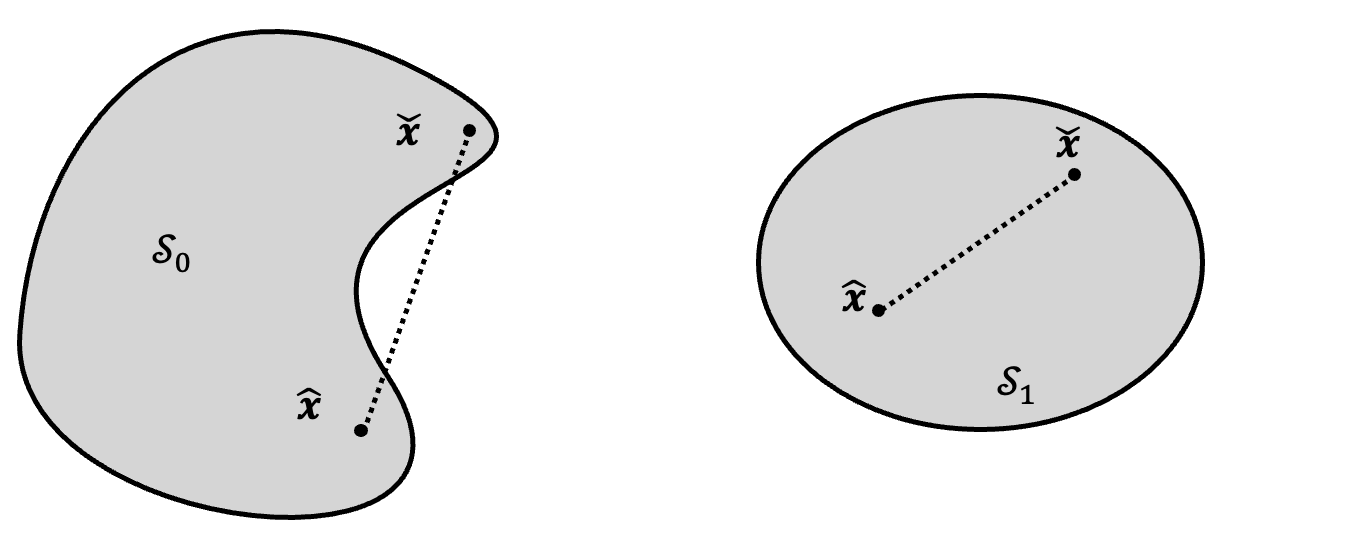
\includegraphics[width=\textwidth, alt={Convex sets}]{figures/convex_sets.png}
    \caption{Set $\mathcal{S}_0$ is not convex, set $\mathcal{S}_1$ is convex.}
    \label{fig:convex_sets}
\end{figure}

A function $f: \mathcal{S} \rightarrow \mathcal{R}$ is termed strictly convex on a convex set $\mathcal{S}$, if 
\begin{equation}
    f(\lambda \hat{\mathbf{x}} + (1-\lambda) \check{\mathbf{x}}) <  \lambda f(\hat{\mathbf{x}}) + (1-\lambda) f(\check{\mathbf{x}}) \quad \forall \hat{\mathbf{x}}, \check{\mathbf{x}} \in \mathcal{S} \quad  \forall \lambda \in [0,1].
\end{equation}
We can asses the convexity of a function $f: \mathcal{S} \rightarrow \mathcal{R}$ on a convex set $\mathcal{S}$ by checking its Hessian $\nabla^2 f$. If the Hessian matrix is positive definite ($\mathbf{y} \cdot \nabla^2 f \cdot  \mathbf{y} > 0 \forall \mathbf{y}$) for all points in $\mathcal{S}$,  $f$ is strictly convex.

\begin{example}{Convex functions}{convexfunctionexample}
    The function $f(\mathbf{x})=x_1^2 + x_2^2$ is convex, as its Hessian \begin{equation}
        \nabla^2f(\mathbf{x}) = 
        \begin{pmatrix}
        2 & 0 \\ 
        0       & 2         
        \end{pmatrix}
    \end{equation} 
    is positive definite. Visually this means, we can draw a line between any two points of the function and it will never intersect the function.

    \includesvg[width =\textwidth]{figures/convex_function_0.svg}
\end{example}


\begin{example}{Non-convex functions}{nonconvexfunctionexample}
    The function $f(x, y)=x_1^4-x_1^2+x_2^2$ is not strictly convex, because its Hessian 
    \begin{equation}
        \nabla^2f(\mathbf{x}) = 
        \begin{pmatrix}
        12x_1^2-2 & 0 \\ 
        0       & 2         
        \end{pmatrix}
    \end{equation} 
    is not positive definite. Visually this means, we can find two points, for which drawing a line between them would cross the function. 
    
    \includesvg[width=\textwidth]{figures/convex_function_1.svg}
\end{example}

An unconstrained optimization problem is termed \emph{convex}, if the objective function $f: \mathcal{S} \rightarrow \mathcal{R}$ is convex and the set $\mathcal{S}$ is convex. If in addition, the set $\mathcal{S}$ is compact (i.e. bounded and closed), there exists exactly one solution for the optimization problem. In conclusion this means, that finding the local minimum in a convex problem is equivalent to finding its global minimum. 

\section{Gradient decent methods}
For analytical convex problems, we only have to find a stationary point (see Equation \ref{eq:stationary_point}) by finding the gradient of the objective function and finding the point where it is vanishing. This requires an explicit differentiable expression of the objective function, which is then rearranged.

However, such an explicit expression of the objective function is not always readily available - e.g. if the objective function is an artificial neural network or a numerical simulation model. In these cases, we are usually just able to compute a local gradient in the vicinity of a point, but are not able to find a closed expression for the gradient. 

An analogy to that would be the search for a minimum in a mountainous landscape with heavy fog: \emph{A person hiking in foggy mountains would be able to only evaluate the height and steepness of the mountains in its close neighborhood. The evaluation of height and steepness takes some time, so the person also wants to find a strategy with a small number of measurements.}

\subsection{Simple steepest decent method}
An obvious approach to minimize such a "foggy" objective function is to follow the steepest gradient direction in order to find a better solution. In the image of searching the lowest point ins a hilly landscape, this is equivalent to descending a mountain by always walking in the direction directly perpendicular to the contour lines. 
A naive algorithm for this can be formulated as follows:
\begin{enumerate}
    \item Pick a starting point $\mathbf{x}^0$.
    \item Calculate the gradient $\nabla f(\mathbf{x}^k)$.
    \item Make a step $\mathbf{x}^{k+1} = \mathbf{x}^k -\eta \nabla f(\mathbf{x}^k)$.
    \item Repeat steps 2 and 3 until you reached a maximum number of iterations $k \le N$ or there is no improvement any more ($ \nabla f(\mathbf{x}^k) < \epsilon$). 
\end{enumerate}
The step itself is scaled with a factor $-\eta \in \mathcal{R}$. The sign stems from the fact that we want to minimize the function. The scaling variable $\eta$ is termed \emph{learning rate} in machine learning contexts and describes how large the step is before reevaluating the gradient again. A smaller learning rate improves convergence of the algorithm towards the exact solution, but requires more steps and more function evaluations. A larger value of $\eta$ makes it harder for the algorithm to converge, as it may "jump" over the minimum or may diverge. 

\begin{example}{Simple steepest decent}{simpledecentexample}
    We want to find the solution of the following quadratic unconstrained optimization problem
    \begin{equation}
        \begin{aligned}
            \min_{\mathbf{x}} \quad & f(\mathbf{x})= (\mathbf{x}-\tilde{\mathbf{x}}) \cdot \mathbf{Q} \cdot (\mathbf{x}-\tilde{\mathbf{x}})
        \end{aligned}
        \label{eq:simpledecent_example}
    \end{equation}
    with 
    \begin{equation}
        \mathbf{Q} = 
        \begin{pmatrix}
        2 & 1 \\
        1 & 1 
        \end{pmatrix}
        \quad \text{and} \quad
        \tilde{\mathbf{x}} = 
        \begin{pmatrix}
        -1\\
        1 
        \end{pmatrix}
        .
    \end{equation}

    The optimization path of a simple steepest decent method with a starting point $\mathbf{x}^0= (4, -1)^\top$ and $\eta=0.1$ is shown in the plot below with a blue line. However, the solution requires quite a lot of iterations.

    \begin{center}
        \includesvg[width=0.5\textwidth]{figures/simple_decent.svg}
    \end{center}   
\end{example}

\subsection{Steepest decent method with incomplete line search}
The previous approach is simple, but requires many repeated evaluations of the multi-dimensional gradient. Instead of going an arbitrary downhill step, it is more efficient to perform a line-search along the search direction to got this step towards the minimum in that direction: 
\begin{enumerate}
    \item Pick a starting point $\mathbf{x}^0$.
    \item Calculate the gradient $\nabla f(\mathbf{x}^k)$ and the search direction $\mathbf{p}^k = - \frac{\nabla f(\mathbf{x}^k)}{\lVert \nabla f(\mathbf{x}^k) \rVert}$.
    \item Solve the sub-problem $\min_{\eta} f(\mathbf{x}^k + \eta \mathbf{p}^k)$ to find the optimal step size $\eta$ for a fixed search direction $\mathbf{p}^k$.
    \item Make a step $\mathbf{x}^{k+1} = \mathbf{x}^k + \eta \mathbf{p}^k$.
    \item Repeat steps 2, 3 and 4 until you reached a maximum number of iterations $k \le N$ or there is no improvement any more ($ \nabla f(\mathbf{x}^k) < \epsilon$). 
\end{enumerate}

The sub-problem is just a one-dimensional optimization problem. However, it still requires an iterative solution, if the resulting function $f(\mathbf{x}^k + \eta \mathbf{p}^k)$ has no analytical expression w.r.t. $\eta$. Hence solving this problem to its exact value still takes some time. We do not need to solve this sub-problem to its exact optimal value, though. We can search for a solution that is "good enough" and save some time. But what is good enough?
There are a couple of criteria to stop an optimization early, one of which is the \emph{Armijo condition} 
\begin{equation}
    f(\mathbf{x}^k + \eta \mathbf{p}^k) \le f(\mathbf{x}^k) + c \eta  \nabla f(\mathbf{x}^k) \cdot \mathbf{p}^k 
\end{equation}
with $c \in (0,1)$. This condition ensures a sufficient decrease of the objective function value assuming that we can expect more decrease if the gradient is larger. 

\begin{example}{Armijo condition}{armijoexample}
    Consider the function $f(x)$ displayed below. The Armijo condition is satisfied in all green ranges.  
    
    \includesvg[width=\textwidth]{figures/armijo_condition.svg}
\end{example}

The Armijo condition is always fulfilled for very small steps, thus we have to consider an additional curvature condition (in combination, these are called \emph{Wolfe conditions}) or implement the condition in a clever way to allow for a sufficiently large step size. Latter can be realized with the \emph{backtracking method}, which is usually used to perform the line search to find the step width: 
\begin{enumerate}
    \item Choose $\eta^0$, e.g. $\eta^0=1$.
    \item Evaluate the Armijo condition $f(\mathbf{x}^k + \eta^k \mathbf{p}^k) \le f(\mathbf{x}^k) + c \eta^k \nabla f(\mathbf{x}^k) \cdot \mathbf{p}^k $
    \item If the condition is fulfilled, we have found a suitable $\eta$, else we try step 2 with a new parameter $\eta^{k+1}=\rho \eta^k$ with a contraction factor $\rho \in (0,1)$ again.
\end{enumerate}
This algorithm usually provides a good compromise, as it provides a sufficiently small step to achieve a valid sufficient decrease, but is still large enough to make reasonable progress towards convergence.

The proposed steepest decent method is a useful strategy for unconstrained optimization problems. However, it can be slow because subsequent search directions are perpendicular to each other and search may take many iterations.

\begin{example}{Steepest decent with incomplete line search}{steepestdecentexample}
    We consider the optimization of Equation \eqref{eq:simpledecent_example} using a steepest decent method with incomplete line search. The optimization path for a starting point $\mathbf{x}^0= (4, -1)^\top$, $\eta^0=5.0$, $c=0.5$, and $\rho=0.8$ is shown in the plot below with a blue line. The solution converges much faster than the simple steepest decent.
    \begin{center}
        \includesvg[width=0.5\textwidth]{figures/steepest_decent.svg}
    \end{center}   
\end{example}

\subsection{Conjugated gradients method}
Especially near the optimum, the steepest decent may lead to a "zig-zag" pattern and many iterations. We can improve the algorithm by ensuring that search directions are conjugated directions to the Hessian of that function. For quadratic problems of the form $f(\mathbf{x}) = \mathbf{x} \cdot \mathbf{A} \cdot \mathbf{x} - \mathbf{b} \mathbf{x}$, this ensures that we can reach the optimum for $\mathbf{x} \in \mathcal{R}^d$ in $d$ steps.

The algorithm of a conjugated gradient method according to Fletchers and Reeves \cite{Fletcher1964} is as follows: 
\begin{enumerate}
    \item Pick a starting point $\mathbf{x}^0$.
    \item Calculate the gradient $\nabla f(\mathbf{x}^k)$.
    \item Compute a conjugate direction $\mathbf{p}^k = -\nabla f(\mathbf{x}^k) + \beta \mathbf{p}^{k-1}$ with  
    \begin{equation}
        \beta = \frac{\nabla f(\mathbf{x}^k) \cdot \nabla f(\mathbf{x}^k)}{\nabla f(\mathbf{x}^{k-1}) \cdot \nabla f(\mathbf{x}^{k-1})}.
    \end{equation}
    \item Solve the sub-problem $\min_{\eta} f(\mathbf{x}^k + \eta \mathbf{p}^k)$ to find the optimal step size $\eta$ for a fixed search direction $\mathbf{p}^k$.
    \item Make a step $\mathbf{x}^{k+1} = \mathbf{x}^k + \eta \mathbf{p}^k$.
    \item Repeat steps 2, 3, 4 and 5 until you reached a maximum number of iterations $k \le N$ or there is no improvement any more ($ \nabla f(\mathbf{x}^k) < \epsilon$). 
\end{enumerate}

\begin{example}{Conjugated gradients}{cgexample}
    We consider the optimization of Equation \eqref{eq:simpledecent_example} using the CG method with incomplete line search for the sub-problem. The optimization path for a starting point $\mathbf{x}^0= (4, -1)^\top$, $\eta^0=5.0$, $c=0.5$, and $\rho=0.8$ is shown in the plot below with a blue line. The solution converges in just two iterations for this 2D problem, as the problem is quadratic.
    \begin{center}
        \includesvg[width=0.5\textwidth]{figures/cg.svg}
    \end{center}   
\end{example}

\subsection{Quasi Newton methods}
Newton's method is a well known method to find roots of a function. 

\begin{example}{Newton's method}{newtonexample}
    Consider the nonlinear function $f(x) = x^2 - 3$ displayed below. To find a root, i.e. the values of $x$ where $f(x)=0$, we can employ Newtons method: 
    \begin{enumerate}
        \item Pick a starting point $x^0$.
        \item Compute the derivative $f'(x)$.
        \item Compute a new point $x^{k+1} = x^k - \frac{f(x^k)}{f'(x^k)}$.
        \item Repeat the steps 2 and 3 until converged.
    \end{enumerate}
    
    \includesvg[width=\textwidth]{figures/netwon_iteration.svg}
    \begin{center}    
        \begin{tabular}{cccc}
    
             Iteration  & $x^k$     & $f(x^k)$  & $f'(x^k)$\\
             \hline
             0          & 3.0       & 6.0       & 6.0\\
             1          & 2.0       & 1.0       & 4.0\\
             2          & 1.75      & 0.0625    & 3.5\\
             3          & 1.7314    & \dots     & \dots\\
        \end{tabular}
    \end{center}
\end{example}


We can utilize Newton's method to find roots of the first derivative of a function, which are stationary points and thus in case of convexity global minima.
We therefore solve the problem 
\begin{equation}
    \nabla f(\mathbf{x}) = \nabla f(\mathbf{x}^k) + \underbrace{\nabla^2 f(\mathbf{x}^k)}_{\mathbf{H}} (\mathbf{x}-\mathbf{x}^k) = 0
\end{equation}
with Newton's iteration procedure 
\begin{equation}
    \mathbf{x}^{k+1} = \mathbf{x}^k  - \mathbf{H}^{-1} \nabla f(\mathbf{x}^k) 
\end{equation}
starting from a starting point $\mathbf{x}^0$. For a quadratic problem, this method would find the solution immediately. However, the inverse Hessian $\mathbf{H}^{-1}$ is computationally expensive to obtain. We use an alternative to computing this term, hence the following method is a "quasi" Newton method. 

We can build up $\mathbf{H}^{-1}$ iteratively in the Broyden-Fletcher-Goldfarb-Shanno (BFGS) \cite{Broyden1970, Fletcher1970, Goldfarb1970, Shanno1970} algorithm: 
\begin{enumerate}
    \item Pick a starting point $\mathbf{x}^0$ and set $(\mathbf{H}^{-1})^0=\mathbf{I}$.
    \item Calculate the gradient $\nabla f(\mathbf{x}^k)$ and compute the direction $\mathbf{p}^k = - (\mathbf{H}^{-1})^0 \nabla f(\mathbf{x}^k)$.
    \item Solve the sub-problem $\min_{\eta} f(\mathbf{x}^k + \eta \mathbf{p}^k)$ to find the optimal step size $\eta$ for a fixed search direction $\mathbf{p}^k$.
    \item Make a step $\mathbf{x}^{k+1} = \mathbf{x}^k + \eta \mathbf{p}^k$.
    \item Compute the difference of gradients $ \mathbf{y}^k = \nabla f(\mathbf{x}^{k+1}) - \nabla f(\mathbf{x}^k)$.
    \item Update the inverse Hessian 
    \begin{equation}
        \nonumber
        (\mathbf{H}^{-1})^{k+1} = 
            \left(\mathbf{I} - \frac{\mathbf{p}^k \otimes \mathbf{y}^k}{\mathbf{p}^k \cdot \mathbf{y}^k} \right)
            \cdot
            (\mathbf{H}^{-1})^k
            \cdot
            \left(\mathbf{I} - \frac{\mathbf{y}^k \otimes \mathbf{p}^k}{\mathbf{p}^k \cdot \mathbf{y}^k} \right) 
            + 
            \frac{\mathbf{p}^k \otimes \mathbf{p}^k}{\mathbf{p}^k \cdot \mathbf{y}^k}
    \end{equation}
    \item Repeat steps 2, 3 and 4 until you reached a maximum number of iterations $k \le N$ or there is no improvement any more ($ \nabla f(\mathbf{x}^k) < \epsilon$). 
\end{enumerate}

\begin{example}{BFGS}{bfgsexample}
    We consider the optimization of Equation \eqref{eq:simpledecent_example} using the BFGS method with incomplete line search for the sub-problem. The optimization path for a starting point $\mathbf{x}^0= (4, -1)^\top$, $\eta^0=5.0$, $c=0.5$, and $\rho=0.8$ is shown in the plot below with a blue line. The solution converges in just two iterations for this 2D quadratic problem.
    \begin{center}
        \includesvg[width=0.5\textwidth]{figures/bfgs.svg}
    \end{center}   
\end{example}


\bibliographystyle{unsrtnat}
\bibliography{literature} 


% https://optimization.cbe.cornell.edu/index.php?title=Main_Page